% Chapter3

\chapter{Building from Previous Work} % Main chapter title

\label{Chapter3} % For referencing the chapter elsewhere, use \ref{Chapter1} 

\lhead{Chapter 3. \emph{Preliminary Design}} % This is for the header on each page - perhaps a shortened title

%----------------------------------------------------------------------------------------
As is mentioned in the introduction, a dynamic energy map has four
major functions: 1) holding, 2) visualizing and 3) analyzing community
level high spatial-temporal resolution energy demand and supply data
4) connection to simulation engine for iterative performance
analysis. 

In the initial instance of Dynamic Energy Map by Baird et al.\
~\cite{baird2014}, function 1) of holding spatial-temporal (although
with low temporal resolution) energy data is realized by processing
the energy simulation data with Microsoft excel and importing the csv
file including ``building name, total conditioned area annual, energy
use intensity, annual and monthly peak demand''. The further
improvement of the current project is to make the geo-database hold
more high resolution energy data, meaning the 8760 hourly energy data
should be contained in the dynamic energy map.

Function 4) of connecting to building simulation data is also realized
by importing simulation result csv files to the geo-database (although
with low temporal resolution).

For function 3), the feasibility analysis of a district energy system
is performed in a stand-alone excel tool~\cite{baird2014} but it is
possible that the analysis result could be linked in to the
geo-database as the energy simulation result. 

For function 2), the spatial and temporal information are visualized
separately in the Lower District Hill Project: the spatial information
of 3D building geometry and location could be visually inspected in
the geo-database but not the hourly energy consumption information. 2)
The temporal visualization of energy demand is done separately in the
excel screening tool as 3D graphs, but no spatial context is present
and the spatial dimension is then lost. The authors thus identified
the crucially missing function: the visualization of such a
spatial-temporal changing of energy behavior as the major goal of the
current project.

\begin{figure}[h!]
  \centering
  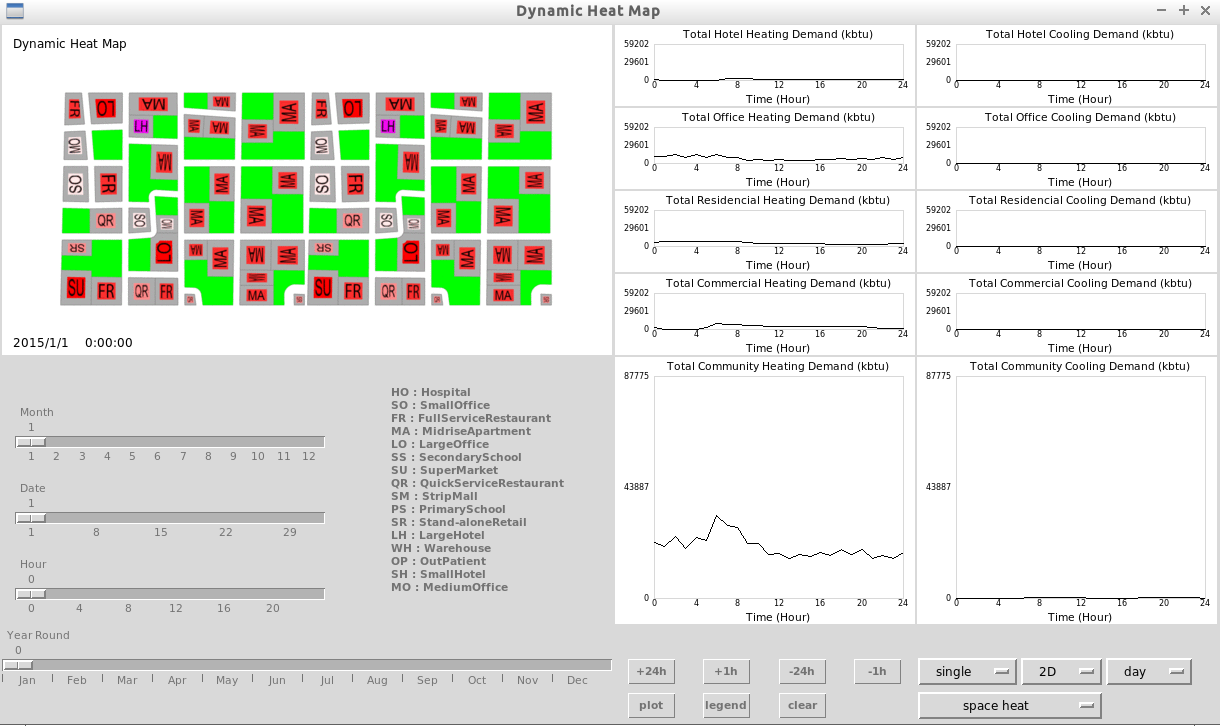
\includegraphics[width=0.7\linewidth]{interface08.png}
  \caption[Dynamic Energy Map Display]{Unified Dynamic Energy Map
    Display System}
  \label{fig:interface08}
\end{figure}